\documentclass[12pt,a4paper, english, titlepage]{article}
\usepackage[utf8]{inputenc}
\usepackage[english]{babel}
\usepackage[T1]{fontenc}
\usepackage{graphicx}
\usepackage{parskip}
\usepackage{siunitx}
%\usepackage{url}
\usepackage[numbers]{natbib}
\usepackage{amsmath} % Needed for split-env in math mode

%\DeclareSIUnit\dbm{{\rm dBm}}
\setlength\belowcaptionskip{5pt}
\newcommand*{\mSIrange}[1][]{\SIrange[range-phrase=\ldots,range-units=brackets,#1]}

\begin{document}

\begin{titlepage}
	\centering
	{\scshape\LARGE NTNU \par}
	\vspace{1cm}
	{\scshape\Large TTT4205 Microwave Techniques \par}
	\vspace{1.5cm}
	{\huge\bfseries Waveguide assignment \par}
	\vspace{2cm}
	{\Large\itshape Magne H. Å. Haneberg \par}
	\vfill
	{\large \today\par}
\end{titlepage}

\section{Rectangular waveguide}

\subsection{Cut-off frequencies}
The cut-off frequency of a hollow waveguide is given by
\begin{equation}
f_{\rm c}^{\rm (mn)} = \frac{c}{2 \pi \sqrt{\epsilon_{\rm r} \mu_{\rm r}}} \sqrt{\left(\frac{m \pi}{a}\right)^{\rm 2} + \left(\frac{n \pi}{b}\right)^{\rm 2}}.
\label{eq:cut-off-waveguide}
\end{equation}
For a \emph{WR75} waveguide, modes $\rm TE_{10}$ and $\rm TE_{20}$, the cut-off frequencies are $f_{\rm c}^{\rm (10)} = \SI{7.8740}{\giga\hertz}$ and $f_{\rm c}^{\rm (20)} = \SI{15.748}{\giga\hertz}$. \par
The unimodal frequency band, $\Delta F$, is given by
\begin{equation}
\Delta F = f_{\rm c}^{\rm (20)} - f_{\rm c}^{\rm (10)} = \SI{7.8740}{\giga\hertz}.
\end{equation}

\subsection{Normalized propagation constants}
The propagation constant of a hollow waveguide is given by
\begin{equation}
k_{\rm z}^{\rm (mn)} = \sqrt{k_{\rm 0}^{\rm 2} \epsilon_{\rm r} \mu_{\rm r} - \left(\frac{m \pi}{a}\right)^{\rm 2} - \left(\frac{n \pi}{b}\right)^{\rm 2}}
\end{equation}
where
\begin{equation}
k_{\rm 0} = \frac{2 \pi f}{c} = \frac{2 \pi f}{\SI{3e8}{\meter\slash\second}}.
\end{equation}
For a \emph{WR75} waveguide, modes $\rm TE_{10}$ and $\rm TE_{20}$, from \SI{5}{} to \SI{25}{\giga\hertz}, the propagation constants are shown in figure \ref{fig:prop_const}.

\begin{figure}[h t b p]
\centering
\includegraphics[width=\textwidth,keepaspectratio]{figures/prop_const.eps}
\caption{Normalized propagation constants in $\rm TE_{10}$ and $\rm TE_{20}$ modes.}
\label{fig:prop_const}
\end{figure}

\subsection{Phase and group velocities}
The phase and group velocities for the $\rm TE_{10}$ mode in the unimodal frequency band is given by equations \ref{eq:phase_v} and \ref{eq:group_v} and plotted in figure \ref{fig:velocity}.

\begin{equation}
V_{\rm ph}^{\rm (mn)} = \frac{\frac{c}{\sqrt{\epsilon_{\rm r} \mu_{\rm r}}}}{\sqrt{1-\left(\frac{f_{\rm c}^{\rm (mn)}}{f}\right)^2}}
\label{eq:phase_v}
\end{equation}
\begin{equation}
V_{\rm g}^{\rm (mn)} = \frac{c}{\sqrt{\epsilon_{\rm r} \mu_{\rm r}}}{\sqrt{1-\left(\frac{f_{\rm c}^{\rm (mn)}}{f}\right)^2}}
\label{eq:group_v}
\end{equation}
\begin{figure}[h t b p]
\centering
\includegraphics[width=\textwidth,keepaspectratio]{figures/velocity.eps}
\caption{Phase and group velocities of ${\rm TE}_{\rm 10}$ wave in the unimodal frequency band}
\label{fig:velocity}
\end{figure}

\subsection{Wave impedance}
The wave impedance of a ${\rm TE}_{\rm mn}$ mode is given by equation \ref{eq:wave_imp}. This impedance is plotted for a ${\rm TE}_{\rm 10}$ wave in figure \ref{fig:wave_imp} for the unimodal frequency band.
\begin{equation}
W_{\rm mn}^{\rm TE} = \frac{\dot E_{\rm x}^{\rm (mn)}} {\dot H_{\rm y}^{\rm (mn)}} = \frac{\omega \mu_{\rm r} \mu_{\rm 0}} {k_{\rm z}^{\rm (mn)}} = \sqrt{\frac{\mu_{\rm r} \mu_{\rm 0}}{\epsilon_{\rm r} \epsilon_{\rm 0}}} \frac{1}{\sqrt{1 - \left(\frac{f_{\rm c}^{\rm (mn)}}{f}\right)^2}}
\label{eq:wave_imp}
\end{equation}

\begin{figure}[h t b p]
\centering
\includegraphics[width=\textwidth,keepaspectratio]{figures/wave_imp.eps}
\caption{Wave impedance of ${\rm TE}_{\rm 10}$ wave in the unimodal frequency band}
\label{fig:wave_imp}
\end{figure}

\subsection{Cut-off frequencies in an ideal dielectric}
The cut-off frequencies for a waveguide is given by equation \ref{eq:cut-off-waveguide}. If the waveguide is filled with air, this corresponds to $\epsilon _{\rm r} = 1$. When filled with a perfect dielectric, $\epsilon _{\rm r}$ changes value. However, it is still a real number. \par
The cut-off frequencies of a \emph{WR75} waveguide filled with a perfect dielectric, $\epsilon _{\rm r} = 2.44$, are shown in table \ref{tab:cut-off-student-nr}.

\begin{table}[h t b p]
\centering
\caption{Cut-off frequencies for waveguide filled with perfect dielectric}
\begin{tabular}{|c|c|} \hline
Mode & Cut-off frequency \\ \hline
${\rm TE}_{\rm 10}$ & \SI{5.0408}{\giga\hertz} \\
${\rm TE}_{\rm 20}$ & \SI{10.082}{\giga\hertz} \\ \hline
\end{tabular}
\label{tab:cut-off-student-nr}
\end{table}

\subsection{Dielectric loss constant}
The dielectric loss constant for a mode ${\rm TE}_{\rm mn}$ is given by equation \ref{eq:dielectric_loss_const}.
\begin{equation}
\alpha _{\rm d}^{\rm (mn)} = \frac{\Delta \bar P _{\rm loss/unit}}{2 \bar P} \approx \frac{\epsilon _{\rm r}''}{\epsilon _{\rm r}'} \frac{\pi}{\lambda} \left(\frac{\Lambda _{\rm mn}}{\lambda}\right)
\label{eq:dielectric_loss_const}
\end{equation}
$\Lambda _{\rm mn}$ and $\lambda$ are given by equations \ref{eq:big-lambda} and \ref{eq:small-lambda}.
\begin{equation}
\Lambda _{\rm mn} = \frac{2 \pi}{k_{\rm z}^{\rm (mn)}} = \frac{\lambda}{\sqrt{1 - \left(\frac{f_{\rm c}^{\rm (mn)}}{f}\right)^2}}
\label{eq:big-lambda}
\end{equation}
\begin{equation}
\lambda = \frac{2 \pi}{k_{\rm 0} \sqrt{\epsilon_{\rm r} \mu_{\rm r}}}.
\label{eq:small-lambda}
\end{equation}
According to \citep{pozar},
\begin{equation}
\epsilon'' = \epsilon' \tan \delta = \epsilon _{\rm r} \epsilon _{\rm 0} \tan \delta.
\end{equation}
Given $\tan \delta = 0.002$, we have
\begin{equation}
\alpha _{\rm d}^{\rm (mn)} \approx \frac{k_{\rm 0} \sqrt{\epsilon_{\rm r} \mu_{\rm r}}}{1000 \sqrt{1 - \left(\frac{f_{\rm c}^{\rm (mn)}}{f}\right)^2}}.
\end{equation}
The dielectric loss constant is plotted for the unimodal frequency band in figure \ref{fig:dielec_loss_const}.
\begin{figure}[h t b p]
\centering
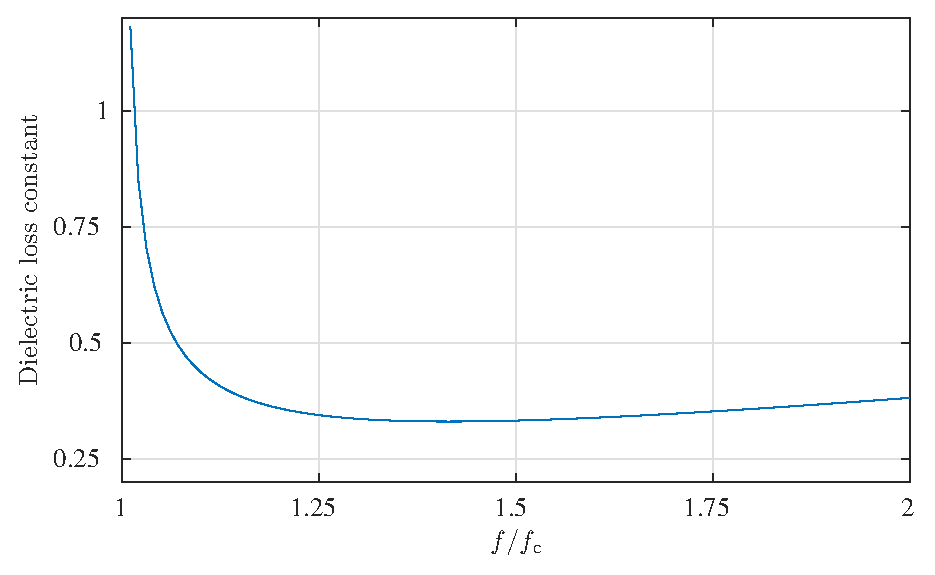
\includegraphics[width=\textwidth,keepaspectratio]{figures/dielec_loss_const.eps}
\caption{Dielectric loss constant, ${\rm TE}_{\rm 10}$ wave.}
\label{fig:dielec_loss_const}
\end{figure}

\section{Microstrip line}

\subsection{Effective permittivity}
The effective permittivity relies on the geometry of the microstrip line.
It is given by equation \ref{eq:eff_perm}.
\begin{equation}
\epsilon_{\rm eff}(f=0) = \left(\frac{\beta}{k_{\rm 0}} \right)^2 = \frac{\epsilon_{\rm r} + 1}{2} + \frac{\epsilon_{\rm r} - 1}{2 \sqrt{1+\frac{10h}{W}}}
\label{eq:eff_perm}
\end{equation}
Given the geometry $h = \SI{1}{\milli\meter}$ and $W = \mSIrange{0.1}{4}{\milli\meter}$, with $\epsilon_{\rm r} = 3.32$, the effective permittivity becomes
\begin{equation}
\epsilon_{\rm eff} = 
\label{eq:eff_perm_calcd}
\end{equation}

\section{Microstrip Branch-Line Directional Coupler}
The \emph{Keysight ADS tools} can be used to calculate the geometry of a microstrip branch-line directional coupler.
Inserting the following values into ADS, the results in table \ref{tab:msbldc_geometry} are obtained.
\begin{itemize}
\item $F_{\rm 0} = \SI{1.6}{\giga\hertz}$
\item $h = \SI{1}{\milli\meter}$
\item $\epsilon_{\rm r} = 3.32$
\item $Z_{\rm 0} = \SI{50}{\ohm}$
\end{itemize}

\begin{table}[h t b p]
\centering
\caption{Branch-line coupler geometry}
\begin{tabular}{|c|c|} \hline
Parameter & Size \\ \hline
${\rm TE}_{\rm 10}$ & \SI{5.0408}{\giga\hertz} \\
${\rm TE}_{\rm 20}$ & \SI{10.082}{\giga\hertz} \\ \hline
\end{tabular}
\label{tab:msbldc_geometry}
\end{table}

\clearpage
\begin{thebibliography}{9}
\bibitem{pozar} David M. Pozar:\\ \emph{Microwave Engineering}\\ Wiley \& Sons,Inc., Fourth ed.
\end{thebibliography}

\end{document}